%%%%%%%%%%%%%%%%%%%%%%%%%%%%%%%%%%%%%%%%%%%%%%%%%%%%%%%%%%%%%%%%%%%%%%
%%	Name: "Signal analysis template"
%%	File name: signalanalysis_template_main
%%	Version: 1.5
%%
%%	Compiler: XeLaTeX
%%
%%%%%%%%%%%%%%%%%%%%%%%%%%%%%%%%%%%%%%%%%%%%%%%%%%%%%%%%%%%%%%%%%%%%%%

\documentclass[conference,compsoc,onecolumn]{IEEEtran}

% *** LANGUAGE UTILITY PACKAGES ***
\usepackage[utf8]{inputenc} % Requerid for including letters with accents
\usepackage[spanish]{babel}



% *** USED PACKAGES ***
% *** MISC UTILITY PACKAGES ***
\usepackage{comment}			% Agregar comentarios
\usepackage{lipsum}				% Inserts dummy text
\usepackage{blindtext}
\usepackage{listings}					% Coding
\usepackage{verbatim}				% Verbatim
\usepackage[final]{pdfpages}
\usepackage{booktabs,dcolumn}
\usepackage{pdflscape}
\usepackage{afterpage}
%\setlist[itemize]{noitemsep, nolistsep}
\usepackage[bookmarks=false]{hyperref}
\usepackage{tcolorbox}									% Coloured boxes, for LATEX examples and theorems, etc
\usepackage{color}
\usepackage{xcolor} % Required for specifying colors by name									% Color packages foreground and back­ground color man­age­men
% *** CITATION PACKAGES ***
\usepackage{cite}
% *** GRAPHICS RELATED PACKAGES ***
\usepackage{graphicx}
\usepackage{caption}
\usepackage{pgfplots}
\usepackage{tikz}
\usetikzlibrary{shapes,arrows}
\usetikzlibrary{decorations.pathmorphing} % noisy shapes
\usetikzlibrary{fit}					% fitting shapes to coordinates
\usetikzlibrary{backgrounds}	% drawing the background after the foreground
\pgfplotsset{compat=1.13}
% *** MATH PACKAGES ***
\usepackage{amsmath}
\usepackage{mathtools}
\usepackage{amssymb}
\usepackage{amsfonts}
\usepackage{expl3}
\usepackage{bm}

% *** SPECIALIZED LIST PACKAGES ***
\usepackage{algorithmic}
\usepackage{listings}					% Coding
\usepackage[framed,numbered,autolinebreaks,useliterate]{mcode}
% *** ALIGNMENT PACKAGES ***
\usepackage{array}
% *** SUBFIGURE PACKAGES ***
%\ifCLASSOPTIONcompsoc
%\usepackage[caption=false,font=normalsize,labelfont=sf,textfont=sf]{subfig}
%\else
%\usepackage[caption=false,font=footnotesize]{subfig}
%\fi
% *** FLOAT PACKAGES ***
\usepackage{fixltx2e}
\usepackage{stfloats}
%\fnbelowfloat
%\usepackage{dblfloatfix}
% *** PDF, URL AND HYPERLINK PACKAGES ***
\usepackage{url}
\usepackage{everypage}


\usepackage{multirow} % In order to be able to insert rows spanning multiple lines
\usepackage{verbatim}
\usepackage[all]{xy}
\usepackage{listings}
\usepackage{subfigure}
\usepackage{multibib}
\usepackage{setspace} 
\usepackage{algorithm}			    	  % To insert nice algorithms

% *** CARPETA DONDE SE GUARDARAN LAS IMÁGENES ***
\graphicspath{{figures/}}

% *** NUEVOS COMANDOS Y CONFIGURACIONES VARIAS ***
\interdisplaylinepenalty=2500
\newcommand{\Lpagenumber}{\ifdim\textwidth=\linewidth\else\bgroup
	\dimendef\margin=0
	\ifodd\value{page}\margin=\oddsidemargin
	\else\margin=\evensidemargin
	\fi
	\raisebox{\dimexpr -\topmargin-\headheight-\headsep-0.5\linewidth}[0pt][0pt]{%
		\rlap{\hspace{\dimexpr \margin+\textheight+\footskip}%
			\llap{\rotatebox{90}{\thepage}}}}%
	\egroup\fi}
\AddEverypageHook{\Lpagenumber}%
\makeatletter
\newcommand{\linebreakand}{%
  \end{@IEEEauthorhalign}
  \hfill\mbox{}\par
  \mbox{}\hfill\begin{@IEEEauthorhalign}
}
\makeatother
\newcommand{\newtxt}[1]{\textcolor{black}{#1}}
\renewcommand\IEEEkeywordsname{Palabras cláve:}
\newcommand{\mx}[1]{\mathbf{\bm{#1}}} % Matrix command
\newcommand{\vc}[1]{\mathbf{\bm{#1}}} % Vector command
\renewcommand{\lstlistingname}{Código}
%% Separación de palabras
\hyphenation{op-tical net-works semi-conduc-tor HHMMSS}


\begin{document}

% *** TITLES AND NAMES ***
% title of the document
\title{Plataforma de seguimiento de datos COVID-19 para Colombia }
% author names and affiliations
\author{
    \IEEEauthorblockN{Juan Sebastian Sierra}
    \IEEEauthorblockA{Escuela de Ciencias Exactas e Ingeniería\\
    Universidad Sergio Arboleda - Bogotá, Colombia\\
    juan.sierra01@correo.usa.edu.co}
    \and
    \IEEEauthorblockN{Leyder Jesus Pacheco}
    \IEEEauthorblockA{Escuela de Ciencias Exactas e Ingeniería\\
    Universidad Sergio Arboleda - Bogotá, Colombia\\
    leyder.pacheco01@correo.usa.edu.co}
    \linebreakand
    \IEEEauthorblockN{Luis Felipe Velasquez}
    \IEEEauthorblockA{Escuela de Ciencias Exactas e Ingeniería\\
    Universidad Sergio Arboleda - Bogotá, Colombia\\
    luis.velasquez01@correo.usa.edu.co}
}
% \begin{flushright}
%   Texto
% \end{flushright}

% *** MAKE TITLE ***
\maketitle
\IEEEoverridecommandlockouts
\IEEEpeerreviewmaketitle

\begin{abstract}
En el presente laboratorio se recolectaran los datos de Covid-19 para colombia y se mostraran estos en diferentes diagramas para entender el comportamiento en el país y en los ciudadanos colombianos, mediante python y sus diferentes librerías. 
\end{abstract}


\begin{IEEEkeywords}
    Python, Covid-19, Datos, OpenData.
\end{IEEEkeywords}


\section{Marco teórico}
\label{sec:introduction}
En esta pandemia, los datos han sido los grandes protagonistas. La crisis ha resaltado la importancia de generar estadísticas oficiales oportunas y confiables para monitores el avance de la enfermedad, detectar grupos vulnerables, medir el impacto de las políticas de aislamiento en la vida de las personas y en la economía, y proyectar las necesidades a futuro.
\singlespacing
En el informe se buscará obtener todos los datos posibles acerca de el Covid-19 en Colombia y como este ha ido evolucionando a través del tiempo, esto se hará mediante gráficas de diferentes tipos para lograr así un seguimiento en diferentes ámbitos del país.
\singlespacing
Inicialmente necesitamos obtener los datos de una fuente confiable y libre, en este caso elegimos \href{https://www.datos.gov.co/}{datos.gov.co} la cual es la pagina de los datos abiertos de Colombia que facilitan la descarga de los datos.
\singlespacing
Estas son :
\begin{enumerate}
    \item \textbf{pandas}: El cual es un paquete de Python que proporciona estructuras de datos similares a los dataframes de R. Pandas depende de Numpy, la librería que añade un potente tipo matricial a Python.
    Pandas proporciona herramientas que permiten:
    \cite{Pandas}.
    \begin{itemize}
        \item leer y escribir datos en diferentes formatos: CSV, Microsoft Excel, bases SQL y formato HDF5
        \item seleccionar y filtrar de manera sencilla tablas de datos en función de posición, valor o etiquetas
        \item fusionar y unir datos
        \item transformar datos aplicando funciones tanto en global como por ventanas
        \item manipulación de series temporales
        \item hacer gráficas
    \end{itemize}
    \item \textbf{Data frames}: Los data frames son estructuras de datos de dos dimensiones (rectangulares) que pueden contener datos de diferentes tipos, por lo tanto, son heterogéneas. Esta estructura de datos es la más usada para realizar análisis de datos\cite{Data}.
        \item \textbf{Numpy}: Es una librería en la que se define un tipo de dato que representa matrices multidimensionales\cite{Data2}.
    \item \textbf{Matplotlib}: Matplotlib es una librería que permite hacer gráficos. Se puede utilizar junto a Numpy o independientemente. Los gráficos pueden ser guardados en ficheros (png, svg, pdf, etc.) o ser utilizados interactivamente. El módulo principal de uso de matplotlib es pyplot\cite{Mat}..
    \item \textbf{SQLite}:Es una base de datos server-less que se puede utilizar en casi todos los lenguajes de programación, incluido Python\cite{SQL}.
\end{enumerate}


\section{Procedimiento}

   
    Para la extracción de los Datos del Covid-19 en Colombia, se obtuvo en la pagina web de datos abiertos de Colombia en www.datos.gov.co donde se encuentran los datos en una plantilla de celdas y de allí se pudo  obtener un link que hace hace referencia a un archivo .csv que contiene todos los datos necesitados
    
            \begin{figure}[H]
            \centering
            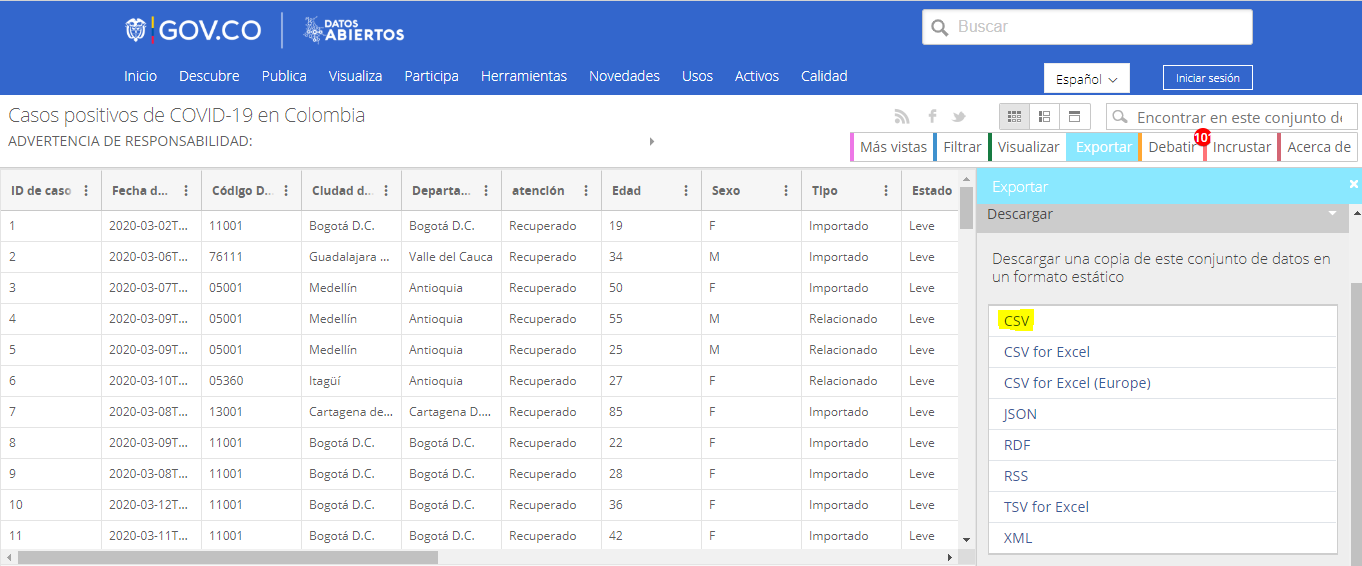
\includegraphics[width=0.75\textwidth]{Figures/Extraccion.PNG}
            \caption{Extracción de datos del Covid-19 en Colombia}
            \label{fig:grafica.png}
        \end{figure}


\label{sec:results}
\singlespacing
La implementación se desarrollo en código python y utilizando su base de datos por defecto mysqlite, ademas se utilizaron dos archivos de python, llamados main.py y myutils.py
 \begin{itemize}
    \item \textbf{Importación de librerías}
    \singlespacing 
    Como primer paso se importo las siguientes librerías las cuales facilitan y ayudan en el proceso
    \lstinputlisting[language=python, firstline=1, lastline=5, caption=Librerias utilizadas para la implementación, captionpos=b, label=lst:SNRCode1]{codigo/main.py}
    \singlespacing
    
    \item \textbf{myutils.py}
    La siguiente sección contiene los códigos utilizado en el archivo myutils.py
    \singlespacing 
    Se descargan los datos con una url e formato CSV
    
    \begin{lstlisting}[language=python, caption=Descarga de datos en formato CSV, captionpos=b, label=lst:SNRCode]
def download_data(url):
    """
    Descarga los datos en formato csv
    """
    return pd.read_csv(url, low_memory=False)
      \end{lstlisting}
    \singlespacing
   
Conexión a la base de datos SQLITE, la cual esta creada como un archivo.bd
        \begin{lstlisting}[language=python, caption=Creación de conexión a la base de datos, captionpos=b, label=lst:SNRCode]
def connect_db(database_name):
    """
    Crea una conexion con la base de datos
    In: database_name - nombre de la base de datos
    Out: conn - conexion, objeto que representa la base de datos.
    """
    conn = None
    try:
        conn = db.connect(database_name)
        print(f'database connected {db.version}')
        return conn
    except Error as e:
        print(e)
        exit(1)
      \end{lstlisting}
    \singlespacing

En esta sección de código se implementó una función que realice un query y retorne su resultado en un DataFrame 
        \begin{lstlisting}[language=python, caption=Funcion del desarrollo de querys, captionpos=b, label=lst:SNRCode]
def make_query(query_statement, conn):
    return pd.read_sql(query_statement, conn)

      \end{lstlisting}
    \singlespacing
  \item \textbf{main.py}
  \singlespacing
 La siguiente sección contiene los códigos utilizado en el archivo main.py, la cual invoca a las funciones de myutils.py para conectarse a la base de datos, ademas de generar las gráficas de estadísticas del Covid-19 en Colombia
                    \singlespacing 
        En esta función se actualizan os datos en caso de que el usuario lo desee, esto lo realiza con el mismo url y la conexión a la base de datos, luego se almacenara en la misma
        \begin{lstlisting}[language=python, caption=Actualización de datos Covid-19, captionpos=b, label=lst:SNRCode]
def update_database(csv_url, conn):
    data = download_data(csv_url)
    print('Datos descargados ...')
    data = rename_columns(data)
    save_data(data, table_name, conn)
    print('Datos almacenados en la base de datos ...')
      \end{lstlisting}
      
        \singlespacing 
En esta función se valida si una tabla existe en la base de datos y se desarrolla  mediante un query que devuelve la respuesta
        \begin{lstlisting}[language=python, caption=Validacion si una tabla existe en la BD, captionpos=b, label=lst:SNRCode]
def exists_table(conn, table_name):
    tables = make_query(
        f"SELECT name FROM sqlite_master WHERE type='table'", conn)
    return tables['name'].str.contains(table_name).any()

      \end{lstlisting}
              \singlespacing 
En esta sección, se invoca a las funciones que grafican las estadísticas del Covid-19 donde recibe y envía a cada una de ellas a conexión y el nombre de la tabla de la base de datos
        \begin{lstlisting}[language=python, caption=Invocación a las funciones graficadoras, captionpos=b, label=lst:SNRCode]
def plot_data(conn, table_name):
    print('Generando las graficas, por favor espere ...')
    torta_por_genero(conn,table_name)
    muertos_por_Depto(conn,table_name)
    activos_por_Depto(conn,table_name)
    recuperados_por_Depto(conn,table_name)
    contagiiados_por_edad(conn,table_name)
    torta_por_Tipo_Contagio(conn,table_name)
      \end{lstlisting}
              \singlespacing 
En el siguiente código se muestran las funciones que dan como resultado una gráfica por cada una de ellas, donde se desarrollaron querys y el resultado del mismo se gráfico mediante la libreria matplotlib:
        \begin{lstlisting}[language=python, caption=Funciones que muestran las estadísticas del Covid-19, captionpos=b, label=lst:SNRCode]


def diarios_comparacion(conn, table_name):
    datainf = make_query(
        f"SELECT strftime('%m-%d', f_notificacion) as mes_not, count(*) as cantidad FROM {table_name} GROUP BY mes_not ORDER BY mes_not", conn)
    datarec = make_query(
        f"SELECT strftime('%m-%d', f_recuperado) as mes_not, count(*) as cantidad FROM {table_name} WHERE mes_not IS NOT NULL GROUP BY mes_not ORDER BY mes_not", conn)
    datamuer = make_query(
        f"SELECT strftime('%m-%d', f_muerte) as mes_not, count(*) as cantidad FROM {table_name} WHERE mes_not IS NOT NULL GROUP BY mes_not ORDER BY mes_not", conn)

    xinf = datainf['mes_not']
    yinf = datainf['cantidad']
    xrec = datarec['mes_not']
    yrec = datarec['cantidad']
    xmuer = datamuer['mes_not']
    ymuer = datamuer['cantidad']

    fig, ax = plt.subplots()
    plt.title('Curva de contagiados en el tiempo(diario)')
    ax.plot(xinf, yinf)
    ax.plot(xrec, yrec)
    ax.plot(xmuer, ymuer)
    plt.legend(['Contagiados', 'Recuperados', 'Muertos'])
    plt.title(
        'Comparacion contagios, recuperados y muertos en el tiempo(diarios')
    # this locator puts ticks at regular intervals
    loc = ticker.MultipleLocator(base=12)
    ax.xaxis.set_major_locator(loc)
    plt.show()

    xinf = datainf['mes_not']
    yinf = datainf['cantidad']
    xrec = datarec['mes_not']
    yrec = datarec['cantidad']
    plt.title('Curva de contagiados')
    fig, ax = plt.subplots()
    ax.plot(xinf, yinf)
    # this locator puts ticks at regular intervals
    loc = ticker.MultipleLocator(base=12)
    ax.xaxis.set_major_locator(loc)
    plt.show()


def torta_por_genero(conn, table_name):
    data = make_query(
        f"SELECT sexo, count(sexo) as cantidad FROM {table_name} WHERE sexo = 'F'  OR sexo = 'M' GROUP BY sexo", conn)
    y = data['cantidad']
    plt.figure()
    plt.title('Procentaje de contagiados por sexo')
    plt.pie(y,
            labels=['Femenino', 'masculino'],
            autopct='%1.1f%%',
            shadow=True)
    plt.show()


def muertos_por_Depto(conn, table_name):
    data = make_query(
        f"select departamento ,count(*) as total from {table_name} WHERE atencion='Fallecido' GROUP BY departamento ORDER BY total", conn)
    dept = data['departamento']
    cont = data['total']
    plt.figure()
    plt.title('Diez Departamentos con mas Fallecimientos')
    plt.barh(dept[-10:], cont[-10:])
    plt.show()


def activos_por_Depto(conn, table_name):
    data = make_query(
        f"select departamento , count(*) as total from {table_name}  GROUP BY departamento ORDER BY total", conn)
    dept = data['departamento']
    cont = data['total']
    plt.figure()
    plt.title('Diez Departamentos con mas Contagiados')
    plt.barh(dept[-10:], cont[-10:])
    plt.show()


def recuperados_por_Depto(conn, table_name):
    data = make_query(
        f"select departamento ,count(*) as total from {table_name} WHERE atencion='Recuperado' GROUP BY departamento ORDER BY total", conn)
    dept = data['departamento']
    cont = data['total']
    plt.figure()
    plt.title('Diez Departamentos con mas recuperados')
    plt.barh(dept[-10:], cont[-10:])
    plt.show()


def contagiiados_por_edad(conn, table_name):
    # Dispersion
    data = make_query(
        f"SELECT edad ,count(*) as total  FROM {table_name}  GROUP BY Edad", conn)
    fig, ax = plt.subplots()
    plt.title('Dispersión por edad de infectados')
    plt.xlabel('Edad(años)')
    plt.ylabel('Infectados')
    ax.scatter(data['edad'], data['total'])
    plt.show()


def torta_por_Tipo_Contagio(conn, table_name):
    data = make_query(
        f"SELECT atencion,count(*) as cantidad FROM {table_name} where atencion !='Recuperado' and atencion !='Fallecido' GROUP BY atencion", conn)
    y = data['cantidad']
    plt.figure()
    plt.title('Porcentaje de atención de contagiados')
    plt.pie(y,
            labels=['', 'En casa', 'Hospital', 'UCI'],
            autopct='%1.1f%%',
            shadow=True)
    plt.show()
      \end{lstlisting}

             \singlespacing 
El contenido de la siguiente función es el que va a ejecutar el usuario, donde puede seleccionar si actualizar nuevamente los datos, o no hacerlo, además de invocar el método que muetsra la gráficas
        \begin{lstlisting}[language=python, caption=Funcion main del programa, captionpos=b, label=lst:SNRCode]


def main(csv_url, database_name, table_name):
    conn = connect_db(database_name)

    if exists_table(conn, table_name):
        print('Los datos ya estan en la base de datos')
        y = input('Desea actualizar la base de datos? ([y]/[n]): ').lower()
        if y == 'y':
            print('Descargando los datos de Covid-19, por favor espere ...')
            update_database(csv_url, conn)
    else:
        print('Descargando los datos de Covid-19, por favor espere ...')
        update_database(csv_url, conn)

    plot_data(conn, table_name)
    close_db(conn)
      \end{lstlisting}
      
        \singlespacing 

        \begin{lstlisting}[language=python, caption=Datos iniciales de la url y archivo de la base de datos SQLITE, captionpos=b, label=lst:SNRCode]

def plot_data(conn, table_name):
if __name__ == '__main__':
    direc_a = os.getcwd()
    print(direc_a)
    csv_url = "https://www.datos.gov.co/api/views/gt2j-8ykr/rows.csv?accessType=DOWNLOAD"
    if 'codes' in direc_a:
        database_name = "datasets/covid.db"
    else:
        database_name = "codes/datasets/covid.db"
    table_name = "covidt"

    main(csv_url, database_name, table_name)
      \end{lstlisting}
\end{itemize}
       
       

\singlespacing
\singlespacing
\section{Resultados}
\label{sec:results}
% Escriba su texto aquí
A partir del procedimiento, se ejecuto el archivo python main.py, el cual descargo el archivo csv  de la pagina de OpenData Colombia, los inserto en una base de datos SQLITE, realiza varias consultas y las gráficas dieron de a siguiente manera:
 
 \begin{enumerate}
     \item Gráfica que representa la curva de contagios por Covid-19
     
                 \begin{figure}[H]
            \centering
            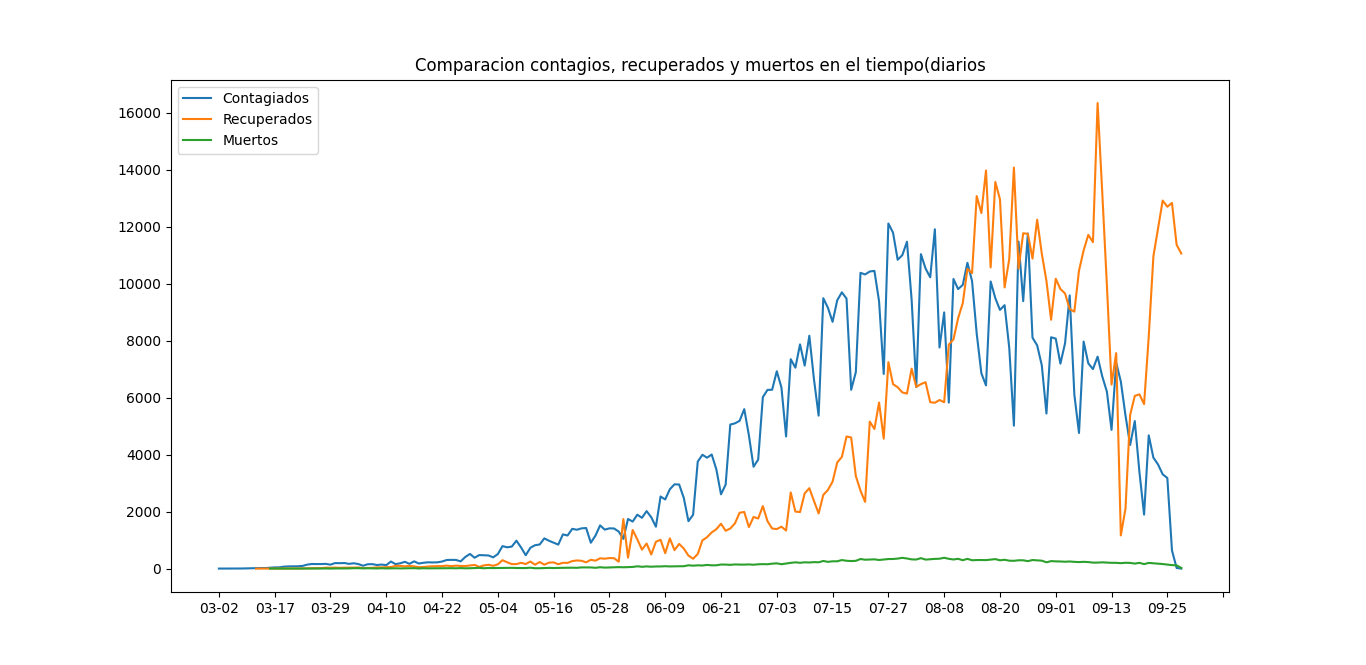
\includegraphics[width=0.75\textwidth]{Figures/CurvaContagios.png}
            \caption{Extracción de datos del Covid-19 en Colombia}
            \label{fig:grafica.png}
        \end{figure}
     
     \newpage
     \item Gráfica de dispersión que demuestra los contagios de Covid-19 por edad
     
                 \begin{figure}[H]
            \centering
            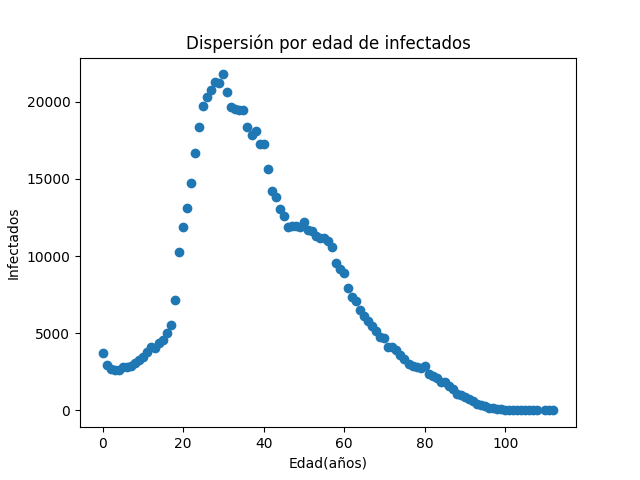
\includegraphics[width=0.6\textwidth]{Figures/InfectadosEdad.png}
            \caption{Extracción de datos del Covid-19 en Colombia}
            \label{fig:grafica.png}
        \end{figure}
     
     \singlespacing
    \item Gráfica de barras con los diez departamentos con mas contagios por covid-19:
     \singlespacing
     
                 \begin{figure}[H]
            \centering
            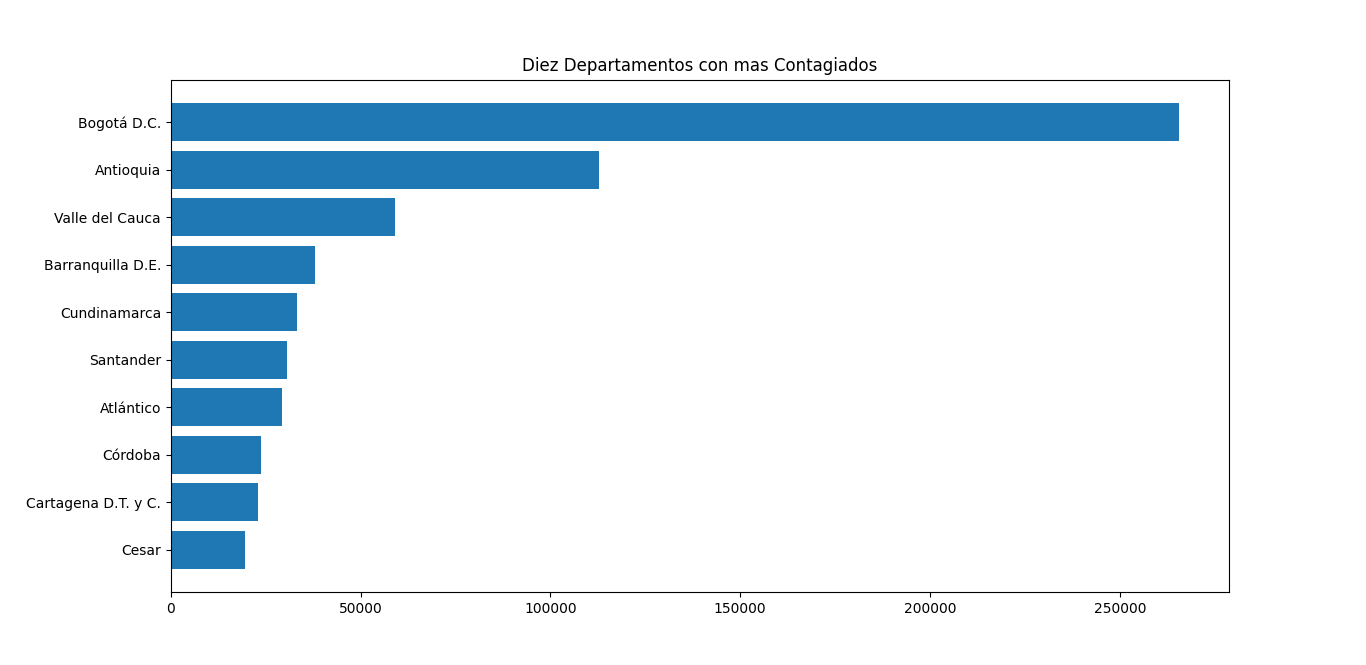
\includegraphics[width=0.75\textwidth]{Figures/ContagiadosDep.png}
            \caption{Extracción de datos del Covid-19 en Colombia}
            \label{fig:grafica.png}
        \end{figure}
    \newpage
    \item Gráfica de barras con los diez departamentos con mas presonas recuperadas por covid-19:
    
                \begin{figure}[H]
            \centering
            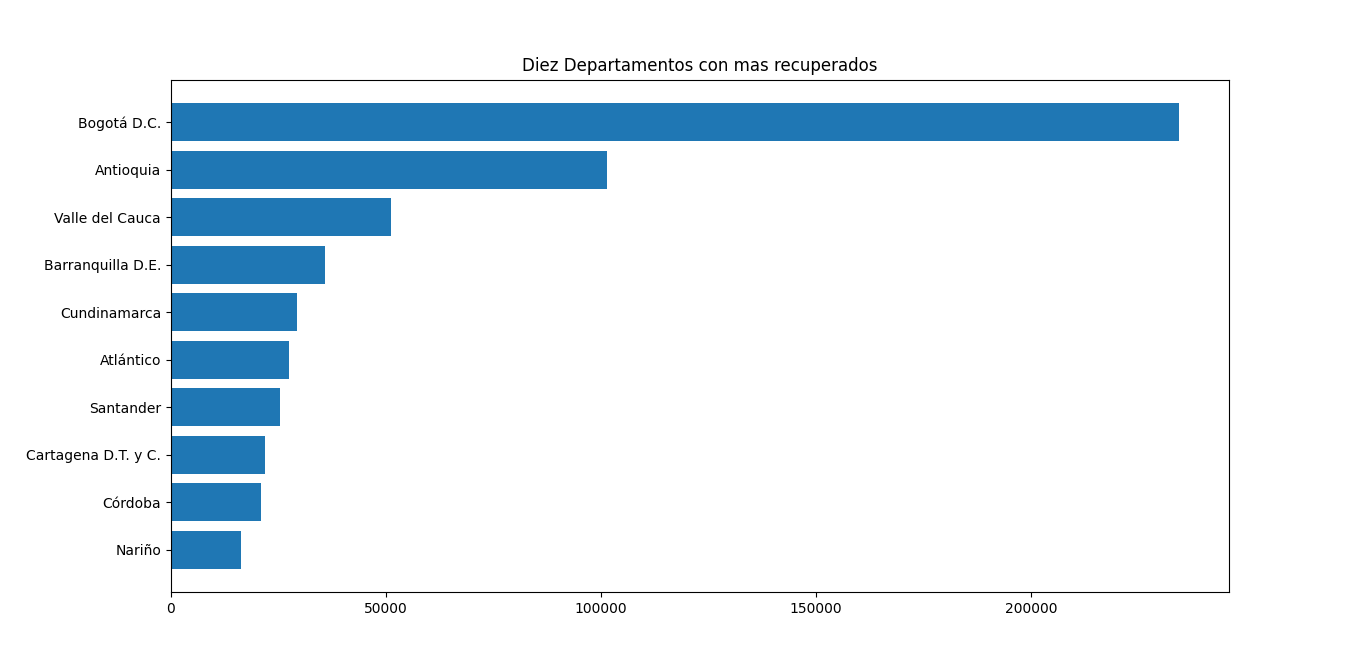
\includegraphics[width=0.75\textwidth]{Figures/RecuperadosDep.png}
            \caption{Extracción de datos del Covid-19 en Colombia}
            \label{fig:grafica.png}
        \end{figure}
    
     \singlespacing
     \item Gráfica de barras con los diez departamentos con mas fallecimientos por covid-19:
     
                 \begin{figure}[H]
            \centering
            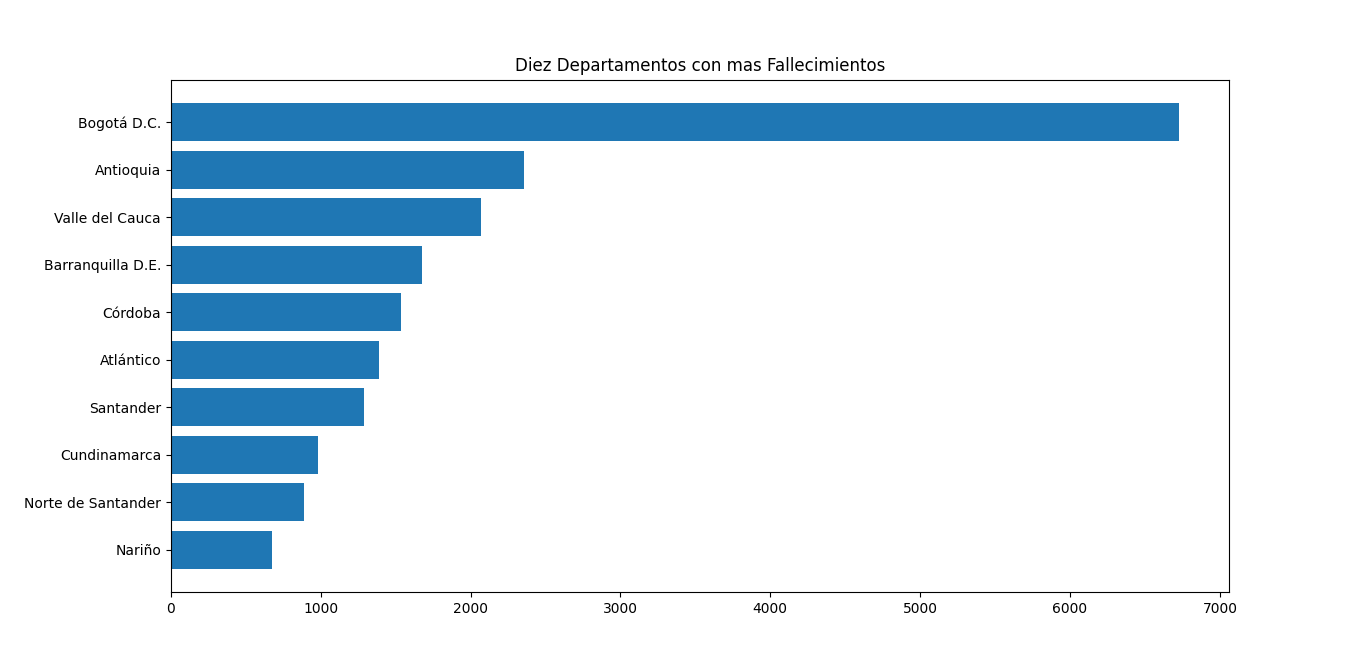
\includegraphics[width=0.75\textwidth]{Figures/FallecidosDep.png}
            \caption{Extracción de datos del Covid-19 en Colombia}
            \label{fig:grafica.png}
        \end{figure}
     
     \singlespacing
     \newpage
        \item Gráfica Tipo Torta que especifica el porcentaje de contagiados por genero:
                    \begin{figure}[H]
            \centering
            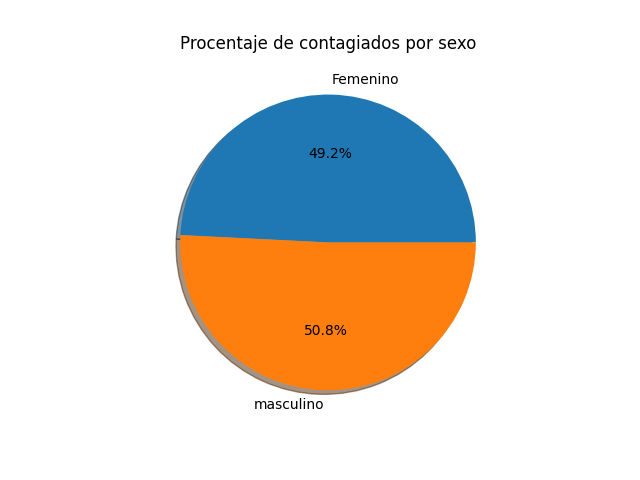
\includegraphics[width=0.7\textwidth]{Figures/ContagiosGenero.png}
            \caption{Extracción de datos del Covid-19 en Colombia}
            \label{fig:grafica.png}
        \end{figure}
        
     \singlespacing
    \item Gráfica Tipo Torta que especifica el porcentaje de cada una de los tipo de atención a las personas contagiadas
    
    
                \begin{figure}[H]
            \centering
            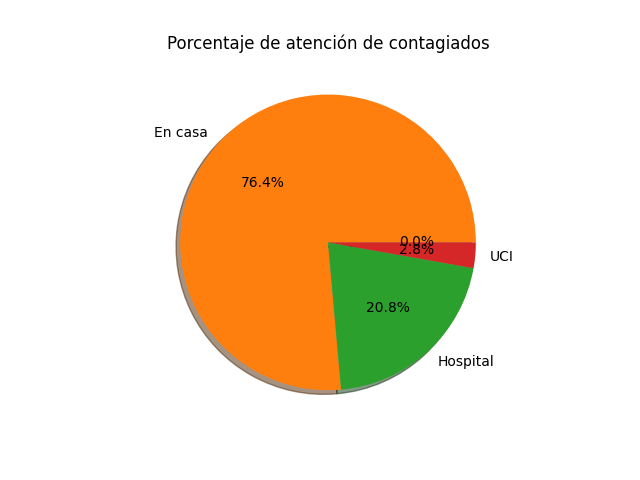
\includegraphics[width=0.7\textwidth]{Figures/atencionContagiados.png}
            \caption{Extracción de datos del Covid-19 en Colombia}
            \label{fig:grafica.png}
        \end{figure}
    
     \singlespacing
 \end{enumerate}



\section{Conclusiones}
\label{sec:conclusions}
Con esta primera parte del proyecto para la creación de una plataforma de seguimiento de datos COVID-19 para Colombia, se logro evidenciar la facilidad con la que se puede extraer datos del internet y poder convertirlos en información visible y útil para las personas. Además, con las tecnologías a disposición como el lenguaje de programación \textit{Python}, el cual facilita y permite automatizar el proceso de extracción y representación de los datos en diferentes tipos de gráficas para tener el conocimiento de los datos de una manera mas clara y concisa.

\textit{Python} cuenta con una gran cantidad de librerías a disposición que permiten realizar diversos programas, especialmente  en la ciencia de datos, librerías como numpy, pandas, matbplotlib, entre otras han permitido que la gran cantidad de datos que se tienen a disposición hoy en día.

\singlespacing
Repositorio del proyecto

\url{https://github.com/SierraJuanSe/COVID_tracker}
\nocite{*}
\bibliographystyle{IEEEtran}
\section{Bibliografia}
\label{sec:biblio}
\bibliography{bib/biblio}




%\pagestyle{empty}
\end{document}


